\documentclass[10pt]{beamer}
\usepackage[utf8]{inputenc}
\usepackage[MeX]{polski}
\usepackage[none]{hyphenat}
\usepackage{ragged2e}
\usepackage{graphicx}
\newcommand{\Csharp}{%
  {\settoheight{\dimen0}{C}C\kern-.05em \resizebox{!}{\dimen0}{\raisebox{\depth}{\#}}}}

\justifying
\emergencystretch=3em
\usetheme{Warsaw}
\title[Projekt systemu do wizualizacji danych w chmurze Azure]{Projekt, implementacja i zautomatyzowane wdrożenie systemu do wizualizacji danych w\,chmurze Azure}
\author{Igor Nowicki}
\institute{

Promotor: dr inż. Jarosław Sikorski\\
Konsultant: mgr Marcin Pytlik	

\bigskip


\includegraphics[width=3.5cm]{./images/WIT-Logo.png}\vskip 0.5cm Studia I stopnia na Wydziale Informatyki, dyplom inżyniera


}
\begin{document}
\maketitle

\begin{frame}
	\frametitle{Agenda}
	\framesubtitle{Plan prezentacji}

	\begin{enumerate}
\item Wstęp
\item Pojęcia
\item Infrastruktura
\item Automatyczne wdrożenie
\item Witryna
\item Wizualizacje
\item Podsumowanie
	\end{enumerate}

\end{frame}

\begin{frame}
\frametitle{Wstęp}
\framesubtitle{Cel pracy}


Niniejsza praca opisuje proces tworzenia strony internetowej w chmurze, z~użyciem narzędzi do wizualizacji danych.

\bigskip

Projekt miał na celu eksplorację dostępnych technologii, z~uwzględnieniem automatyzacji procesów wdrożeniowych.

\end{frame}

\begin{frame}
	\frametitle{Pojęcia}
	\framesubtitle{Podstawowe terminy}

	\begin{itemize}
		\item \textbf{Chmura obliczeniowa}: model świadczenia usług przetwarzania danych przez Internet,
		\item \textbf{Azure}: platforma chmurowa firmy Microsoft,
		\item \textbf{Bank Światowy}: międzynarodowa instytucja finansowa zajmująca się udzielaniem pożyczek krajom rozwijającym się.
	\end{itemize}
\end{frame}

\begin{frame}
	\frametitle{Infrastruktura}
	\framesubtitle{Usługi chmury}
	Na infrastrukturę rozwiązania składały się usługi: 

	\bigskip
	
	\begin{itemize}
		\item \textbf{Azure App Service}: usługa hostowania aplikacji internetowych,
		\item \textbf{Azure SQL}: zarządzanie bazami danych,
		\item \textbf{Azure Active Directory}: przyznawanie dostępu do zasobów,
		\item \textbf{Power BI App}: aplikacja do wizualizacji danych.
	\end{itemize}

	\bigskip

	\begin{figure}
		\centering
		\begin{minipage}{.15\linewidth}
			\centering
			
\includegraphics[width=0.9\linewidth]{./images/App-Services.png}
		\end{minipage}\hfill
		\begin{minipage}{.15\linewidth}
			\centering
			
\includegraphics[width=0.9\linewidth]{./images/SQL-Database.png}
		\end{minipage}\hfill
		\begin{minipage}{.15\linewidth}
			\centering
			
\includegraphics[width=0.9\linewidth]{./images/Active-Directory.png}
		\end{minipage}\hfill
		\begin{minipage}{.15\linewidth}
			\centering
			
\includegraphics[width=0.9\linewidth]{./images/Power-BI.png}
		\end{minipage}
	\end{figure}
\end{frame}

\begin{frame}
	\frametitle{Automatyczne wdrożenie}
	\framesubtitle{Skrypty PowerShell}
	
Skrypty wdrożeniowe wykorzystywały następujące narzędzia:

\bigskip

\begin{itemize}
	\item \textbf{PowerShell}: język skryptowy stworzony przez firmę Microsoft,
	\item \textbf{Terraform}: narzędzie typu Infrastruktura jako Kod,
	\item \textbf{PowerShell Az}: biblioteka do zarządzania zasobami w Azure,
	\item \textbf{Power BI REST API}: interfejs programistyczny Power BI App.
\end{itemize}

\bigskip

\begin{figure}
	\centering
	\begin{minipage}{.15\linewidth}
		\centering
		
\includegraphics[height=4.1em]{./images/powershell.png}
	\end{minipage}\hfill
	\begin{minipage}{.15\linewidth}
		\centering
		
\includegraphics[height=4em]{./images/terraform.png}
	\end{minipage}\hfill
	\begin{minipage}{.15\linewidth}
		\centering
		
\includegraphics[height=6em]{./images/powershell-az.png}
	\end{minipage}\hfill
	\begin{minipage}{.15\linewidth}
		\centering
		
\includegraphics[height=4em]{./images/power-bi-rest-api.png}
	\end{minipage}
\end{figure}

\end{frame}

\begin{frame}
	\frametitle{Witryna}
	\framesubtitle{Projekt ASP.NET}
	Przy przygotowaniu witryny użyłem frameworka ASP.NET Core MVC wraz z szablonami Razor. 

	\bigskip

	Do stworzenia witryny zostały użyte:

	\bigskip

	\begin{itemize}

		\item \textbf{\Csharp{}},
		\item \textbf{ASP.NET Core MVC},
		\item \textbf{Entity Framework Core}.
	\end{itemize}

	\bigskip

	\begin{figure}
		\centering
		\begin{minipage}{.30\linewidth}
			\centering
			
\includegraphics[width=0.5\linewidth]{./images/c_sharp.png}
		\end{minipage}\hfill
		\begin{minipage}{.30\linewidth}
			\centering
			
\includegraphics[width=0.5\linewidth]{./images/asp_net_core_mvc.png}
		\end{minipage}\hfill
		\begin{minipage}{.30\linewidth}
			\centering
			
\includegraphics[width=0.5\linewidth]{./images/ef_core.png}
		\end{minipage}
	\end{figure}
\end{frame}

% \begin{frame}
% 	\frametitle{Witryna}
% 	\framesubtitle{Architektura MVC}
% 	Framework ASP.NET Core MVC wykorzystuje architekturę, w której istnieje podział na trzy główne komponenty:
	
% 	\smallskip

% 	\begin{itemize}
% 	\item \textbf{Model danych}: klasy reprezentujące przetwarzane dane,
% 	\item \textbf{Widok}: warstwa prezentacji w postaci szablonów Razor,
% 	\item \textbf{Kontroler}: moduł zarządzający przetwarzaniem zapytań.
% 	\end{itemize}


% 	\smallskip

% 	\begin{figure}
% 		\centering
% 		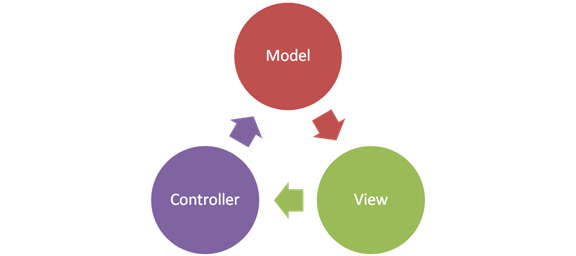
\includegraphics[width=0.8\linewidth]{./images/mvc.png}
% 	\end{figure}

% \end{frame}

\begin{frame}
	\frametitle{Witryna}
	\framesubtitle{Strona internetowa}

	Na witrynę składają się następujace elementy:

	\bigskip	

	\begin{itemize}
		\item \textbf{Ankieta}: zestaw pytań z wiedzy na temat rozwoju świata,
		\item \textbf{Prezentacja wyników}: statystyki odpowiedzi na pytania,
		\item \textbf{Prezentacja danych}: osadzone wykresy z Power BI App,
		\item \textbf{Panel administracyjny}: moduł do szybkich zmian w treści.
	\end{itemize}
\end{frame}

\begin{frame}
	\frametitle{Podsumowanie}
	\framesubtitle{Podsumowanie}
	Projekt pozwolił mi na rozeznanie się w technologiach używanych w~procesach związanych z chmurą obliczeniową. 
	
	\bigskip

	Sprawdzono następujące narzędzia:
	
	\bigskip
	
	\begin{itemize}
		\item \textbf{Terraform} do definiowania infrastruktury w chmurze, 
		\item \textbf{PowerShell} do automatyzacji zadań,
		\item \textbf{Azure App Service} do hostowania aplikacji, 
		\item \textbf{Azure SQL} do zarządzania bazą danych,
		\item \textbf{Power BI} do prezentacji danych.
	\end{itemize}
	
	\bigskip
	
	Praca ta może służyć jako punkt wyjścia do bardziej zaawansowanych projektów w środowisku chmury obliczeniowej w przyszłości.	
\end{frame}

\begin{frame}
	\frametitle{Dziękuję za uwagę}
	\framesubtitle{Pytania?}
	
	\centering
	\huge{Dziękuję za uwagę.}
\end{frame}

\end{document}